\chapter{Approximation of FEA results by polynomial functions}
\label{chapter:approximation}

%The method of approximation of output from the Finite element method is based on premise, that computer memory and performance are limited. Without some kind of simplification or compression no program can efficiently process large amount of data generated by extensive finite element analysis.

This chapter contains the description of the proposed method for approximation of results from the Finite element method, which are discrete values, by polynomial functions. It is an alternative to the compression method and representation of the data introduced in chapters \ref{chapter:data-management} and \ref{chapter:SVD}. It is worth noting that this method was excluded from the final implementation of the desktop post-processor because of the hard-to-control error of approximation and unfavorable performance characteristics. The content of this chapter is also published in \cite{Benes2016} and \cite{Benes2016Pollack}.

%----------------------------------------------------------------------------------------
%	SECTION Idea
%----------------------------------------------------------------------------------------

\section{Idea}

The multigrid method \cite{Briggs2000,Shaidurov2013,Hackbusch2013} was the inspiration for this work. Multigrid method allows to solve partial differential equations using the hierarchy of domain discretizations. The main idea of multigrid method is to make the convergence of iterative method faster due to global corrections of error that is made from time to time on the coarser mesh. There are many variations of multigrid method. However, all of them need existence of mesh hierarchy that represents domain discretizations of different mesh sizes.

Basic steps of multigrid method are:

\begin{itemize}
    \item \textbf{Smoothing} -– The main goal of the smoothing phase is the high-frequency error reduction. It can be done e.g. by few iterations of the Gauss-Seidel method.
    \item \textbf{Restriction} -- Restriction of the residual from the finer to the coarser mesh.
    \item Solution of the coarse problem.
    \item \textbf{Prolongation} -- Interpolation and projection of the correction computed on the coarser mesh to the finer mesh.
\end{itemize}

The main problem with a mesh hierarchy is that often none is available. Only the finest mesh exists. The coarser meshes must be either generated directly by a mesh generator \cite{Frey2000,Rypl1998} in the pre-processing phase or it must be created from the finer mesh. But generating coarser mesh from the finer one is very problematic or even impossible, because corresponding nodes between different levels should be preserved to be sure that multigrid method will work correctly without special modifications.

Therefore, it was decided to do visualization of the results from the finite element analysis on the fine mesh that is used for solution of FEM. Different methods of simplification and compression of the resulting data in space and time were developed and data were projected back to fine mesh. Results of the projection and comparison of methods are presented in this paper.

%----------------------------------------------------------------------------------------
%	SECTION Implementation
%----------------------------------------------------------------------------------------

\section{Implementation}

Even if the mesh hierarchy is generated, one of the obstacles for using the same multigrid techniques as are often used in the finite element analysis is that only one mesh hierarchy is available. That is sufficient for finite element solver, because this hierarchy is used to solve only one set of equations. However, in the post-processor it is necessary to display various kinds of data, such as temperature, displacements, stress, strain, etc. These quantities are scalars, vectors or tensors of second order. Components of vectors and tensors could be considered in post-processing as a scalar and therefore scalars will be dealt in the following text. Every scalar is represented in the finite element analysis by a set of discrete values computed in nodes or Gauss points, but in the strong formulation of a problem, it is a function. For graphical purposes, it is possible and often suitable to replace the set of discrete values by a continuous function. In the following text, the set of discrete values describing a scalar will be denoted as the discrete function or original function, but approximation of the discrete values for graphical purposes by continuous function will be called approximation function (shape functions used in FEM are not used here).

Approximation functions should be as simple as possible to be representable by a small set of parameters. Therefore, the domain of approximation function should respect the character of the discrete function. It can’t be the whole mesh, because one part of mesh could contain data replaceable by a simple linear function and other part could have much wilder character. It is therefore necessary to find alternative division of problem domain that will respect the shape of function in space and time better than the mesh hierarchy used in the multigrid method. Moreover, each quantity component must have its separately generated mesh hierarchy.

%----------------------------------------------------------------------------------------
%	SUB-SECTION Octree generation
%----------------------------------------------------------------------------------------

\subsection{Octree generation}

Domain space has to be divided into subdomains of the size which allows to replace discrete function with continuous, simpler, e.g. linear function that is easy to describe by fewer parameters. The goal is to automatically recognize areas in mesh, where the nature of function is smooth (the function is continuous together with the first derivatives and very coarse mesh can be used) and areas in which function rapidly changes its character (the first derivatives are large or the function is even discontinuous). These areas of interest become object of further subdivision, because for visualization purposes they need finer underlying mesh. For recursive division of 3D space the octree data structure is suitable (see Figure \ref{fig:octree-visualization}). The other spatial dividing data structures used in computer graphics were investigated, but octree seemed to be the best choice due to its hierarchical form and low average depth.

\begin{figure}[H]
\centering
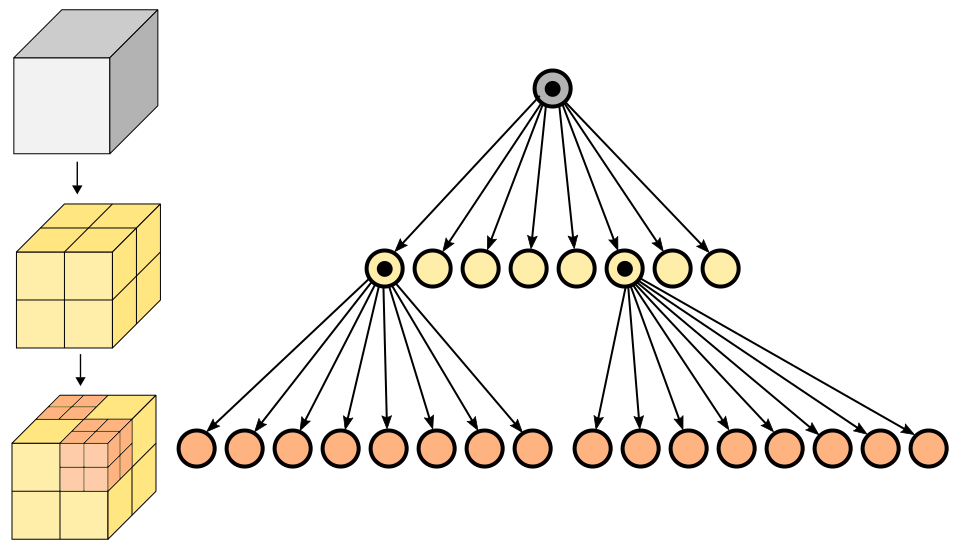
\includegraphics[width=0.8\textwidth]{figures/chapter-approximation/figure1}
\decoRule
\caption[Octree visualization]{Octree visualization. Left: Recursive subdivision of a cube into octants. Right: The corresponding octree.}
\label{fig:octree-visualization}
\end{figure}

Basic overview of the decomposition and approximation procedure is in Listing \ref{alg:approximation}. At first whole mesh is inserted into one big cube -- octree root node. Then a condition that tells whether to divide current domain into eight subdomains is needed. Three conditions were designed. All have to be satisfied to proceed with decomposition.

\begin{enumerate}
    \item First condition specifies minimum number of finite element nodes to be represented by single octree cell. There are two reasons. Firstly, some specification of minimum number is necessary to compute approximation function, e.g. least square trilinear algorithm needs at least 8 values. Secondly, if the number is too small and the approximation function does not fit ideally, subdivision of the octree will be too subtle and memory consumption will easily exceed the case with no approximation applied at all.
    \item Second condition is based on maximal allowed relative error of chosen approximation function. Algorithm that replaces discrete data points with continuous approximation function also calculates relative error of the method. This number is then compared with some preset fixed value. According to the experiment results the most appropriate value of 1\% was chosen.
    \item Third condition describes maximum depth of octal tree. Each level of the tree exponentially increases memory consumption of data values stored in octree. Maximum depth is therefore artificially set to some acceptable value, e.g. 9. However, this depth should not be reached in common cases, it is ensured by condition 1.
\end{enumerate}

If all conditions are met, domain represented by the current octree node is divided into eight subdomains. Differences between original value of discrete function and value of approximation function in the same point are transferred to corresponding sub-nodes based on their location and whole process is recursively repeated in all octree sub-nodes. The difference $D_i$ of the $i$-th data value is defined by

\begin{equation}
D_i=V_i-\bar{V}_i, % or \overline ?
\end{equation}

where $V_i$ is the original function value in the $i$-th node and $\bar{V}_i$ is the value of approximation function in the same location as the $i$-th node.

Similar procedure -- passing residuals between mesh levels -- is applied in the multigrid method. Due to this approach the top levels of octree filter out main character of function (lower frequencies), bottom levels and leaves of the octree catch higher frequencies of function values.

%----------------------------------------------------------------------------------------
%	SUB-SECTION Approximation in space
%----------------------------------------------------------------------------------------

\subsection{Approximation in space}
\label{sec:approximation-in-space}

Discrete values within an octree cell are replaced by a continuous function which is as simple as possible and can be represented in memory by a few parameters. It is therefore necessary to find suitable type of function and in the case of polynomial functions also the order of the function. Compression algorithm has to be very fast. Compromise between low error and memory consumption must be found. For the sake of simplicity at the beginning of the work the relations between neighboring octree nodes were neglected. Nodal values in each octree cell are approximated separately.

The compression procedure requires the surface representation of the mesh to be already created. The element connectivity and nodal coordinates has to be present in memory and accessible in constant $\mathrm{O}(1)$ time. Efficient methods to create this surface representation are described in Chapter \ref{chapter:mesh-visualization} and also in \cite{Benes2015}.

The procedure is reading the FEM results divided to data sets from the external file and then processing the data sets one by one. By a data set is meant primarily the array of floating-point numbers corresponding to one component of one quantity, e.g. $x$ component of displacement vector, temperature (which is scalar) or one component of stress tensor. Each floating-point number is the value of the quantity in single time step corresponding to one node or gauss-point. Whole array is loaded from file into computer memory, its values are distributed into growing octree and the approximation is calculated and saved in corresponding octree cells. After that the original data are deleted and algorithm continues with the next data component.

Compression has to be made on-the-fly during loading of data from the file to the memory between each data component. Starting compression after all results has been loaded to the memory would not make sense, because the main purpose of the compression step is to save overall memory consumption of the post-processor. Therefore, the format of data should ideally be designed in the way that each data component is separated in single data file or at least in one isolated data block in the file not mixed with other data. No particular order of data components is required. However, data formats used by common finite element software packages are usually designed in the way that the components of each quantity are grouped together. We rely mainly on GiD postprocess file format (\file{.res}) described in detail in \cite{GiDPostProcess} where data are divided to blocks according to physical quantity and time step. Each block is the list of value tuples introduced by a node number (or element number in case of values in gauss-points), e.g. $x$, $y$ and $z$ component triplet for displacement vector in node $42$ in time step $3.0$. To avoid multiple passes through the data file the value tuples are cached and processed right after reading the whole data block.

\begin{lstlisting}[caption=Core of aproximation procedure,label=alg:approximation]
function OctreeInternalNode.InsertDataValues(dataValues, dataComponentId, depth, approximationMethod)
{
  // find approximation function and save it in current octree node
  approximation = ComputeApproximation(dataValues, dataComponentId, approximationMethod)
  DataCatalog[dataComponentId] = approximation
  // if condition #2 is met, propagate values to child nodes
  if (approximation.MaxRelativeError > MIN_RELATIVE_ERROR_TO_EXPAND)
  {
    // split residual values to octants based on data point positions
    foreach (dataValue in dataValues)
    {
      // calculate residual and distribute to octants according to position
      position = mesh.Nodes[dataValue.NodeId].Position
      residual = dataValue.Value - approximation.GetValueAt(position)
      octantIndex = getIndexOfOctantOnPosition(position)
      residuals[octantIndex].Add(new DataValue(residual, dataValue.NodeId))
    }
    foreach (octantIndex in range 1..8)
    {
      // if condition #1 is met, algorithm is recursively called on child octree node
      if (residuals[octantIndex].Count > max(MIN_LEAF_DATA_POINTS_COUNT, approximationMethod.MinNumberOfDataPoints))
      {
        // recursive call to InsertDataValues, if children[octantIndex] is LeafNode, than recursion is stopped
        children[octantIndex].InsertDataValues(residuals[octantIndex], dataComponentId, depth + 1, approximationMethod)
        // if child node is leaf, find out if expansion is needed
        if (children[octantIndex] is LeafNode)
        {
          // if condition #3 is met, algorithm can continue with octree node expansion
          if (depth < MAX_OCTREE_DEPTH - 1)
          {
            // if condition #2 is met, expand leaf node
            if (children[octantIndex].DataCatalog[dataComponentId].MaxRelativeError > MIN_RELATIVE_ERROR_TO_EXPAND)
            {
              children[octantIndex] = new OctreeInternalNode(children[octantIndex].LowerBounds, children[octantIndex].UpperBounds)
              children[octantIndex].InsertDataValues(residuals[octantIndex], dataComponentId, depth + 1, approximationMethod)
            }
          }
        }
      }
    }
  }
}

function OctreeLeafNode.InsertDataValues(dataValues, dataComponentId, depth, approximationMethod)
{
  // find approximation function and save it in current octree node
  DataCatalog[dataComponentId] = ComputeApproximation(dataValues, dataComponentId, approximationMethod)
}

function ComputeApproximation(dataValues, dataComponentId, approximationMethod)
{
  switch (approximationMethod)
  {
    case TrilinearInterpolation:
      approximation = DoLeastSquaresTrilinearInterpolation(dataValues)
    ...
  }
  // compute absolute error
  maxError = 0;
  foreach (dataValue in dataValues)
  {
    position = mesh.Nodes[dataValue.NodeId].Position
    error = dataValue.Value - approximation.GetValueAt(position)
    maxError = Max(maxError, Math.Abs(error));
  }
  approximation.MaxError = maxError;
  approximation.MaxRelativeError = maxError / GlobalDataRange[dataComponentId]
  return approximation
}    
\end{lstlisting}

After loading a data block, compression is started. Listing \ref{alg:approximation} contains pseudo-code of recursive procedure that is the core of the compression algorithm. Figure \ref{fig:octree-generation} contains overview of this algorithm in form of UML Activity diagram. The input is an array of nodal values in one component of one field defined on the mesh in single time step. In case of data stored in gauss-points the values has to be at first extrapolated to nodes using natural coordinates supplied in the data file. Nodal data are then passed as an input parameter \code{dataValues} to the function \code{InsertDataValues} that is called upon the octree root node which represents one big cube that surrounds the whole mesh. Each \code{dataValue} object is a structure consisting of floating-point number Value and integer \code{NodeId} that represents a key to the table of nodes in global mesh object. \code{InsertDataValues} is pure virtual function declared in abstract base class \code{OctreeNode} and its implementation differs in derived classes. Its implementation in \code{OctreeLeafNode} is straightforward and so follows description of its implementation in class \code{OctreeInternalNode}. Simplified class diagram of the key types involved in Listing \ref{alg:approximation} is shown in Figure \ref{fig:octree-class-diagram}.

\begin{figure}[H]
\centering
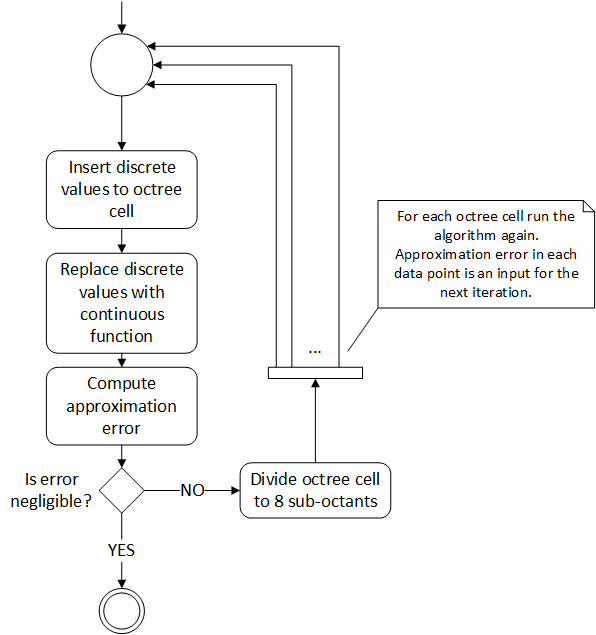
\includegraphics[width=0.8\textwidth]{figures/chapter-approximation/figure2}
\decoRule
\caption[Octree generation]{Octree generation algorithm in form of activity diagram.}
\label{fig:octree-generation}
\end{figure}

\begin{figure}[H]
\centering
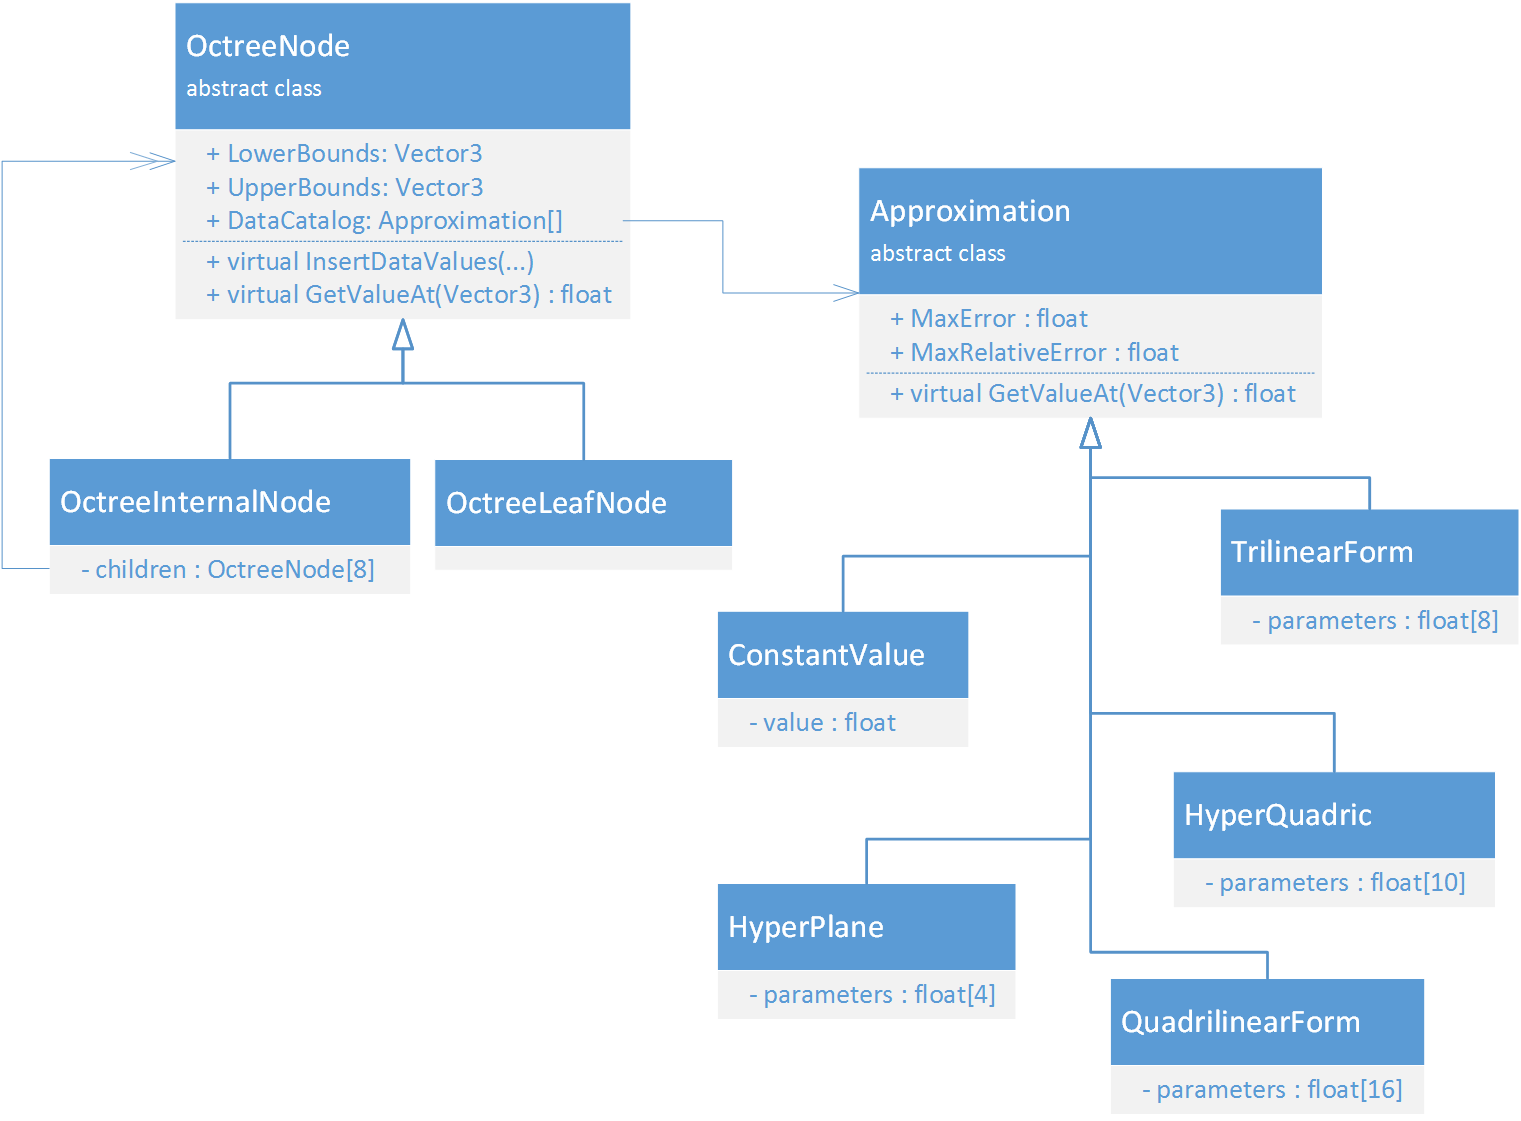
\includegraphics[width=\textwidth]{figures/chapter-approximation/figure3}
\decoRule
\caption[Diagram of octree generation classes]{Class diagram of types involved in octree generation algorithm.}
\label{fig:octree-class-diagram}
\end{figure}

At first the algorithm computes parameters of continuous approximation function of discrete data values provided (variable \code{approximation}). In case of trilinear interpolation it uses least square method to calculate 8 parameters of a polynomial regression model and stores them in \code{DataCatalog} table which is a property of each octree node. Then the maximal relative approximation error is computed.

Approximation function for data values in the octree cell is assessed with the help of several metrics. First, absolute approximation error, which is the difference between the original nodal value and the value of approximation function, is evaluated in all nodes. Then, relative approximation error is obtained by dividing the absolute approximation error by global range of values (difference between global maximum and global minimum of original nodal values). The maximum relative approximation error in an octree cell is one of three parameters (see condition 2 above) that are used by the algorithm to decide whether to proceed with further subdivision of the octree cell. These three parameters control the overall quality of approximation, memory consumption and performance and need to be fine-tuned during testing on real-world data.

If the maximal approximation error is too high, the algorithm continues, calculates approximation error in each node and stores it in table residuals in relevant octant according to its position in current octree cell. \code{residuals} is a table of data value arrays and it is a local variable that will be disposed after each call to function \code{InsertDataValues} finishes. Algorithm then iterates over all child octants and checks for number of residuals assigned to them. If condition 1 stated above holds, algorithm is recursively called upon each child octree cell. If the octree cell is a leaf node, recursion is stopped and algorithm determines whether it should split current leaf octree cell into 8 sub-segments by checking conditions 2 and 3. In other words, if the current octree branch is not deep enough and maximal residual belonging to current child octree cell is higher than designated epsilon value, then this leaf cell is replaced with internal cell and function \code{InsertDataValues} is called upon this new \code{OctreeInternalNode} object. Residuals located in current octant are passed as an input to this function.

This continues until approximation of current data component is good enough in all octree cells.  When the algorithm finishes, original discrete data can be deleted, because the created octree structure with approximation functions in its nodes is all that is needed to reconstruct the original data. Then the algorithm can proceed with reading and processing next data set. Note that these operations are to a considerable extent independent and processing of data sets can be parallelized. However, if the same octree data structure is reused for multiple data sets, then the access to \code{DataCatalog} and octree node expansion has to be synchronized using standard locking mechanisms.

Also note that passing residuals of approximation instead of original data between octree levels is important, because it allows to describe the main character of function (lower frequencies) on top levels and details (high-frequency changes) on bottom levels of the octree. This design is inspired by the Multigrid method basic principles.

%----------------------------------------------------------------------------------------
%	SUB-SUB-SECTION Approximation functions
%----------------------------------------------------------------------------------------

\subsubsection{Approximation functions}

Various approximation functions were investigated and tested. Besides polynomial functions also Discrete cosine transform \cite{Roma2011} and Wavelet transform \cite{Li2014} were considered. Since the data compression algorithm has to be very fast, simple polynomial approximation functions were preferred. They are summarized below:

\begin{itemize}
  \item \textbf{Mean value} -- A single value (average value) replaces the set of discrete values. Arithmetic mean was used during testing because it is fast to compute unlike the median. Also, it takes into account whole spectrum of values in contrast of the mode value that is the value that occurs most often in the collection. It is suitable in statistics where the measurement errors have to be excluded. However, in the case of the results from the FEM the user wants to see extremes in data and these outlying results should be rather highlighted instead of truncated. That is the reason why is neither the arithmetic mean nor other statistically estimated mean value suitable for this purpose. Mean value approximation diagram is depicted in Figure \ref{fig:mean-value-approx}.

  \begin{figure}[H]
  \centering
  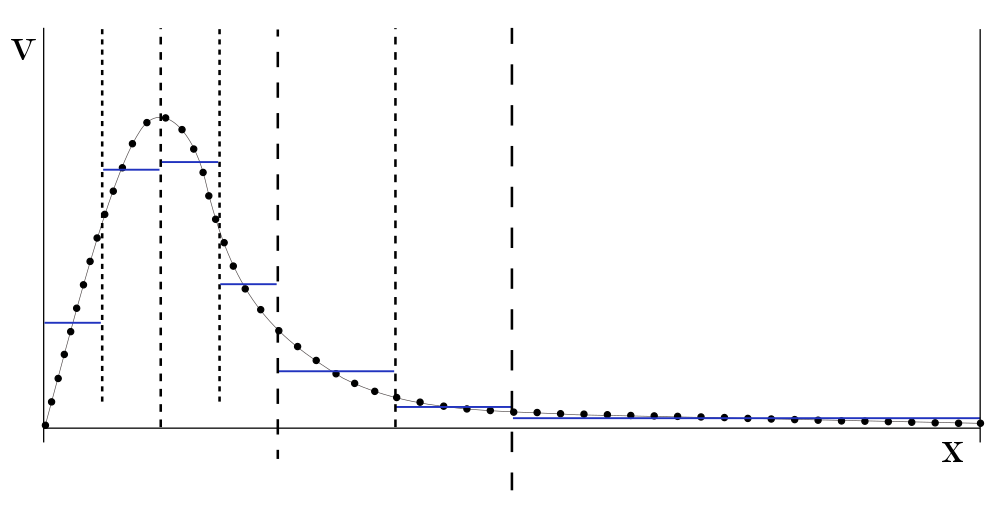
\includegraphics[width=\textwidth]{figures/chapter-approximation/figure4}
  \decoRule
  \caption[Mean value approximation diagram]{Mean value approximation diagram. Dashed lines denote octree division process. Shorter the line the deeper subdivision represents. Mean value is not suitable because of high errors and discontinuities between approximation cells. $v$ stands for function value and $x$ for spatial dimension.}
  \label{fig:mean-value-approx}
  \end{figure}

  \item \textbf{Regression} -- Finds a polynomial that models relationship between a scalar dependent variable and one or more explanatory (independent) variables. In three-dimensional problem there are three independent variables. Polynomial regression models are often fitted using the least squares method. The implementation used in this work is based on solving linear system of equations using LU decomposition. Key thing is that the size of the system does not depend on the number of data values, but on the number of approximation function parameters. Therefore, the algorithm has linear computational complexity and scales well. Several polynomials were tested. In the functions below $x$, $y$, $z$ are spatial coordinates, $c_i$ are parameters which determine the shape of the polynomial and $v$ is the function value.

  \begin{itemize}
    \item \textbf{Linear} -- Hyperplane, only four parameters per octree cell. Value $v$ in the point with coordinates $x$, $y$, $z$ is computed using linear interpolation function in the form
    
    \begin{equation}
    v=c_{1}x + c_{2}y + c_{3}z + c_{4}.
    \end{equation}
    
    Figure \ref{fig:octree-creation} contains example of creation of octree node hierarchy driven by this function.
    
    \item \textbf{Quadratic} -- Parametric shape models known as Hyperquadrics. They have too many parameters per cell (10) and are not suitable to capture continuity between octree cells. Value v in the point with coordinates $x$, $y$, $z$ is computed using quadratic interpolation function in the form

    \begin{equation}
      v=c_{1}x^2 + c_{2}y^2 + c_{3}z^2 + c_{4}xy + c_{5}xz + c_{6}yz + c_{7}x + c_{8}y + c_{9}z + c_{10}.
    \end{equation}

    \item \textbf{Trilinear} -- 8 parameters, the best compromise, consistent with neighboring octree cells, almost “seamless” transitions between octree cells. Also used in the FEM. Value $v$ in the point with coordinate $x$, $y$, $z$ is computed using trilinear interpolation function in the form
    
    \begin{equation}
      v=c_{1}xyz + c_{2}xy + c_{3}xz + c_{4}yz + c_{5}x + c_{6}y + c_{7}z + c_{8}.
    \end{equation}

    The least squares method is applied to find parameters $c_{1},...,c_{8}$. The problem is solved by minimizing the sum of squared residuals $G$ of the linear regression model

    \begin{equation}
      G = \sum_{i=1}^{N}(v_i - (c_{1}x_{i}y_{i}z_{i} + c_{2}x_{i}y_{i} + c_{3}x_{i}z_{i} + c_{4}y_{i}z_{i} + c_{5}x_{i} + c_{6}y_{i} + c_{7}z_{i} + c_{8}))^2,
    \end{equation}
    
    where $N$ is number of values which are interpolated. When the parameters of interpolation are known, value in any point of the approximated volume can be found simply by providing $x$, $y$, and $z$ coordinates of the point in the equation.
    
    \item \textbf{Tri-quadratic} -- Too many describing parameters with no significant benefit over trilinear form.
    
    \item \textbf{Quadrilinear form} -- Generalized trilinear form, extended by temporal dimension, only theoretical option, not implemented.
    

  \end{itemize}

\end{itemize}

\begin{figure}[!tbp]
  \centering
  \begin{minipage}[b]{0.4\textwidth}
    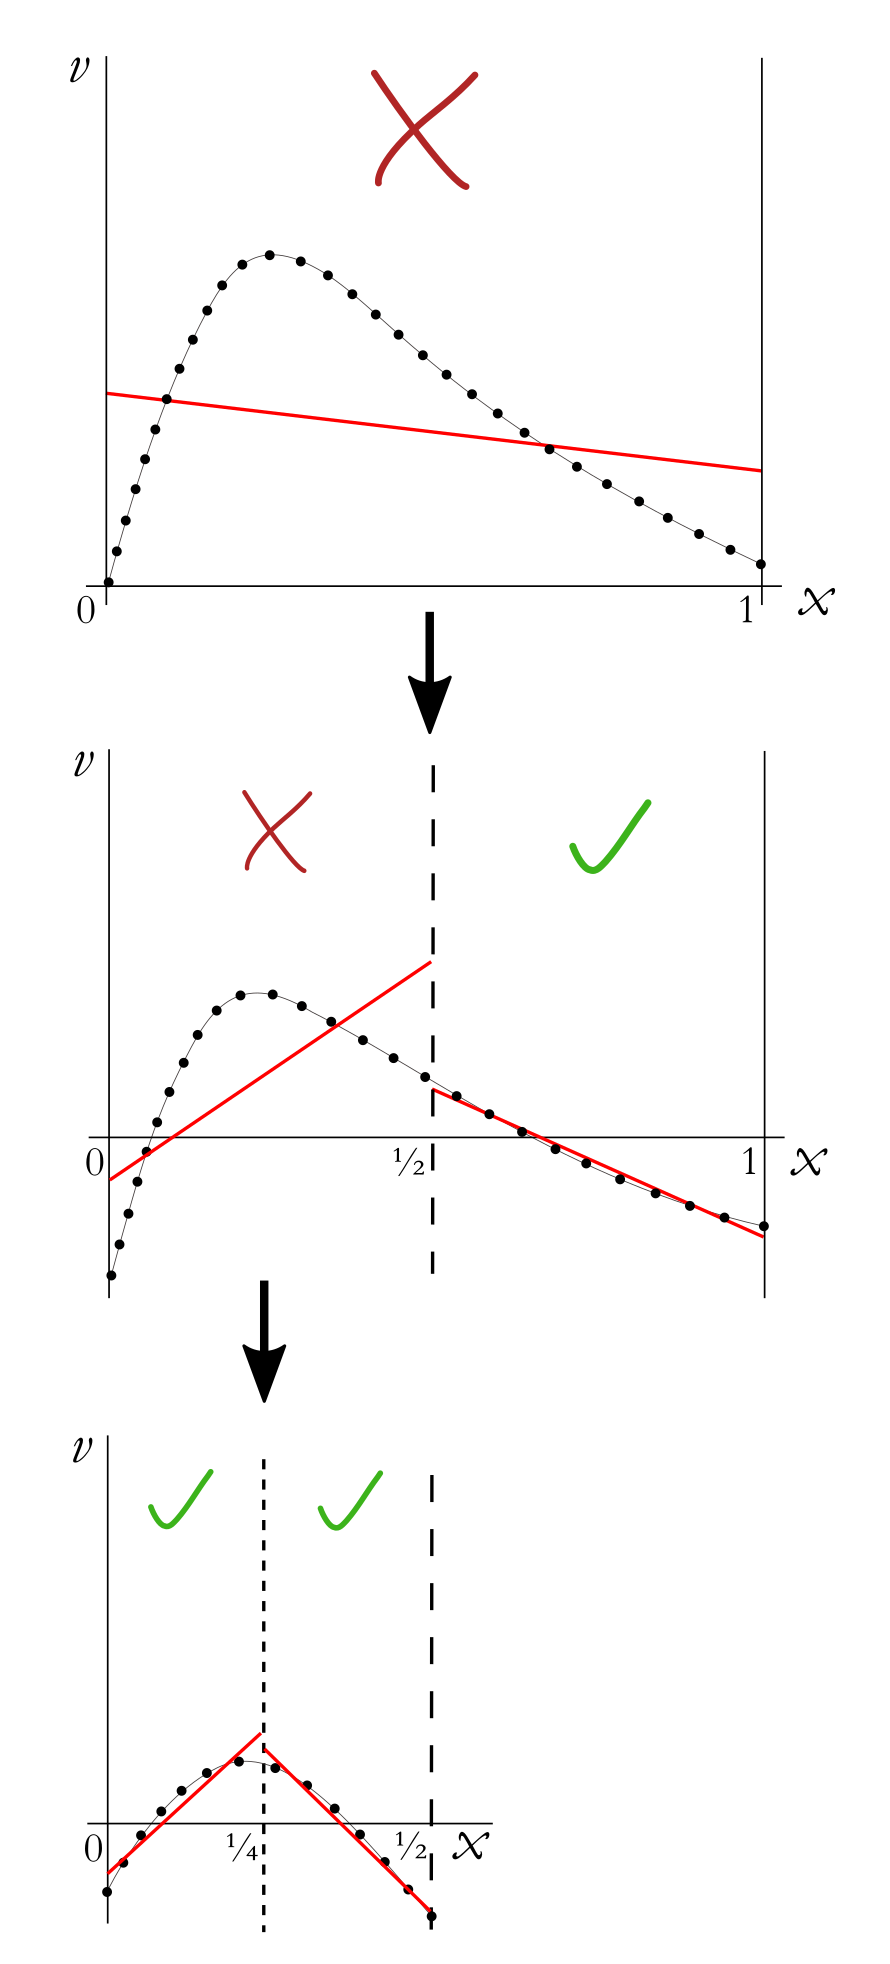
\includegraphics[width=\textwidth]{figures/chapter-approximation/figure5}
    \rule{\textwidth}{.4pt}
    \captionsetup{width=\linewidth}
    \caption[Octree creation]{Octree creation example based on linear approximation error.}
    \label{fig:octree-creation}
  \end{minipage}
  \hfill
  \begin{minipage}[b]{0.4\textwidth}
    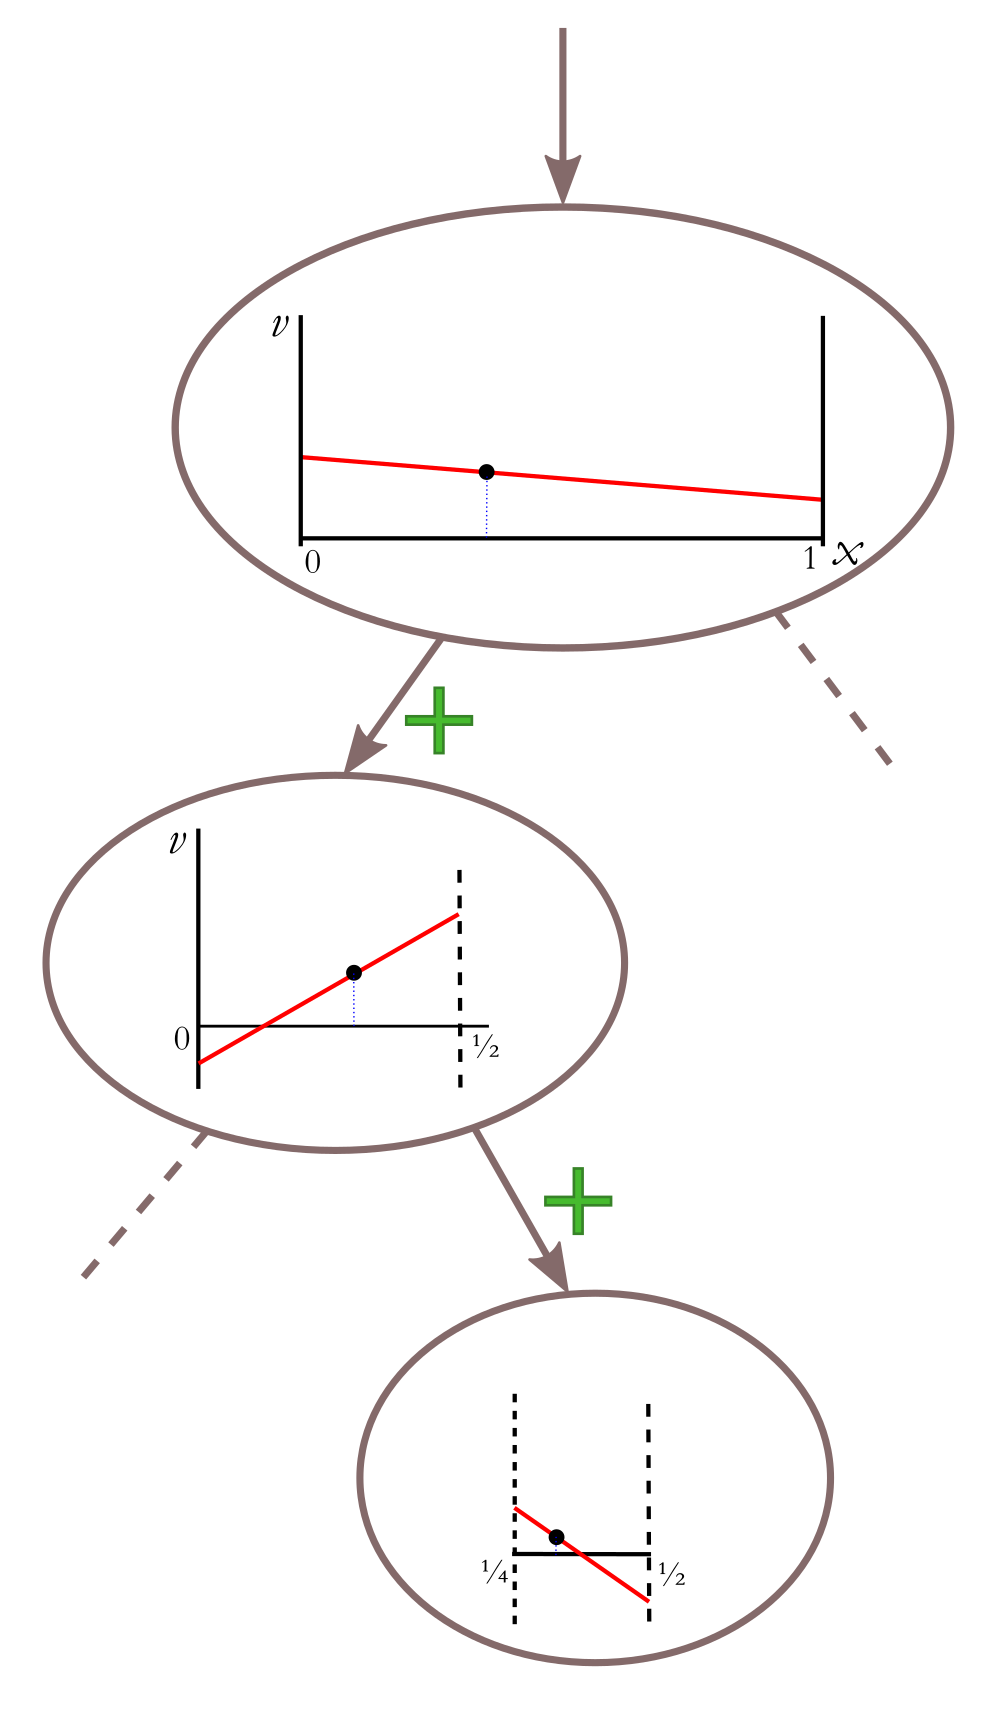
\includegraphics[width=\textwidth]{figures/chapter-approximation/figure6}
    \rule{\textwidth}{.4pt}
    \captionsetup{width=\linewidth}
    \caption[Nodal value computation]{Nodal value computation diagram.}
    \label{fig:nodal-value-computation}
  \end{minipage}
\end{figure}

Figure \ref{fig:nodal-value-computation} depicts computation of nodal value via traversing octree from the root to the leaves and simultaneously summing up approximation errors. Root node of the octree contains all data components in all time steps where data value of an arbitrary element node can be computed. If an approximation is not sufficiently accurate in current octree node, correction can be made with the help of data stored in lower levels of the octree and summing up corrections together with initial value to compute final value for the node.

%----------------------------------------------------------------------------------------
%	SUB-SUB-SECTION Results
%----------------------------------------------------------------------------------------

\subsubsection{Results}

The benchmark is designed to compare maximal relative approximation error, average error and compression ratio when using different approximation methods. Two test data sets were chosen (Figure \ref{fig:reactor-vessel-displacements} and Figure \ref{fig:reactor-containment-displacements}), both contain displacement vector values with three components ($u$, $v$ and $w$) and about 30 time steps. Maximal relative approximation error is the highest relative error of an approximation method in single element node across all data components and time steps. Average error is a weighted sum of approximation errors in all nodes and data components divided by the number of these approximations. Compression ratio is memory consumption of the proposed data representation divided by memory consumption of original post-processor that does not use any data approximation techniques. Results are summarized in Table \ref{tab:reactor-vessel-results} and Table \ref{tab:reactor-containment-results}.

\begin{figure}[H]
\centering
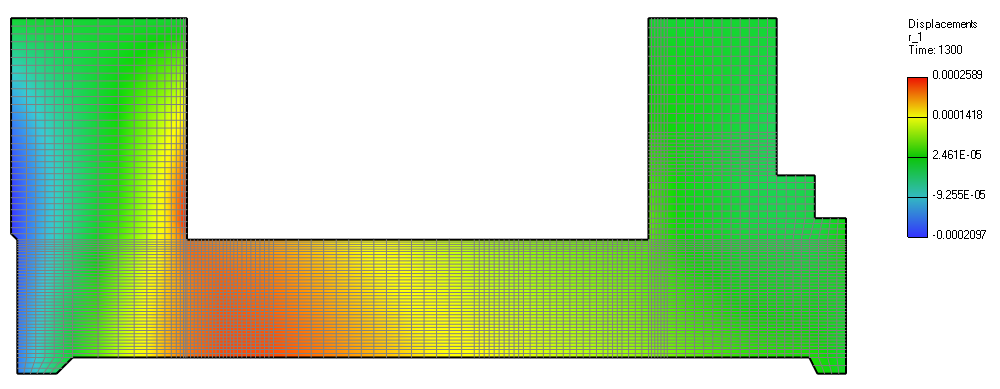
\includegraphics[width=\textwidth]{figures/chapter-approximation/figure7}
\decoRule
\caption[Reactor vessel 2D]{Reactor vessel 2D. Displacements visualization.}
\label{fig:reactor-vessel-displacements}
\end{figure}

\begin{table}[H]
\caption[Approximated results of reactor vessel 2D simulation]{Reactor vessel 2D. Spatial octree approximation results.}
\label{tab:reactor-vessel-results}
\centering
\begin{tabular}{| l | r | r | r |}
\hline
\tabhead{ } & \tabhead{Max error [\%]} & \tabhead{Average error [\%]} & \tabhead{Compression ratio [\%]} \\
\hline
Mean value & 75.28 & 0.6268 & 55.3\\
Linear regression & 44.23 & 0.1842 & 17.7\\
Trilinear regression & 81.27 & 0.1751 & 16.9\\
\hline
\end{tabular}
\end{table}

\begin{figure}[H]
\centering
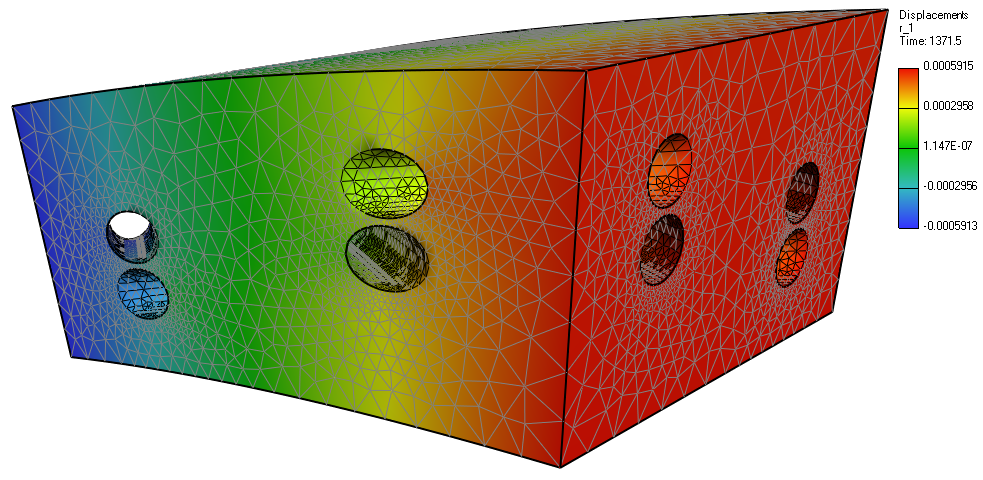
\includegraphics[width=\textwidth]{figures/chapter-approximation/figure8}
\decoRule
\caption[Segment of reactor containment]{Segment of reactor containment. Displacements visualization.}
\label{fig:reactor-containment-displacements}
\end{figure}

\begin{table}[H]
\caption[Approximated results of reactor containment simulation]{Segment of reactor containment. Spatial octree approximation results.}
\label{tab:reactor-containment-results}
\centering
\begin{tabular}{| l | r | r | r |}
\hline
\tabhead{ } & \tabhead{Max error [\%]} & \tabhead{Average error [\%]} & \tabhead{Compression ratio [\%]} \\
\hline
Mean value & 38.62 & 1.667 & 63.1\\
Linear regression & 32.9 & 0.305 & 59.4\\
Trilinear regression & 89.46 & 0.2237 & 56\\
\hline
\end{tabular}
\end{table}

\begin{figure}[H]
\centering
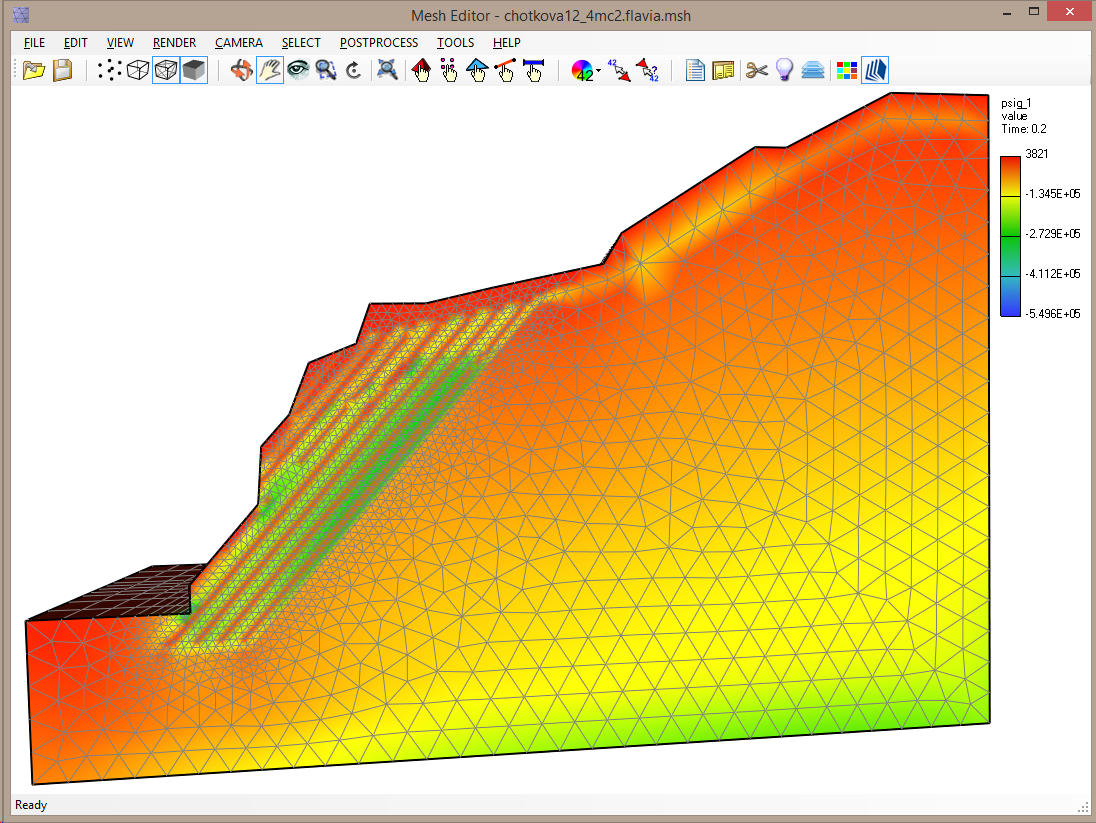
\includegraphics[width=\textwidth]{figures/chapter-approximation/figure9}
\decoRule
\caption[Geological layers simulation results]{Geological layers simulation results. Exact data values, no approximation applied.}
\label{fig:geological-layers-exact}
\end{figure}

\begin{figure}[H]
\centering
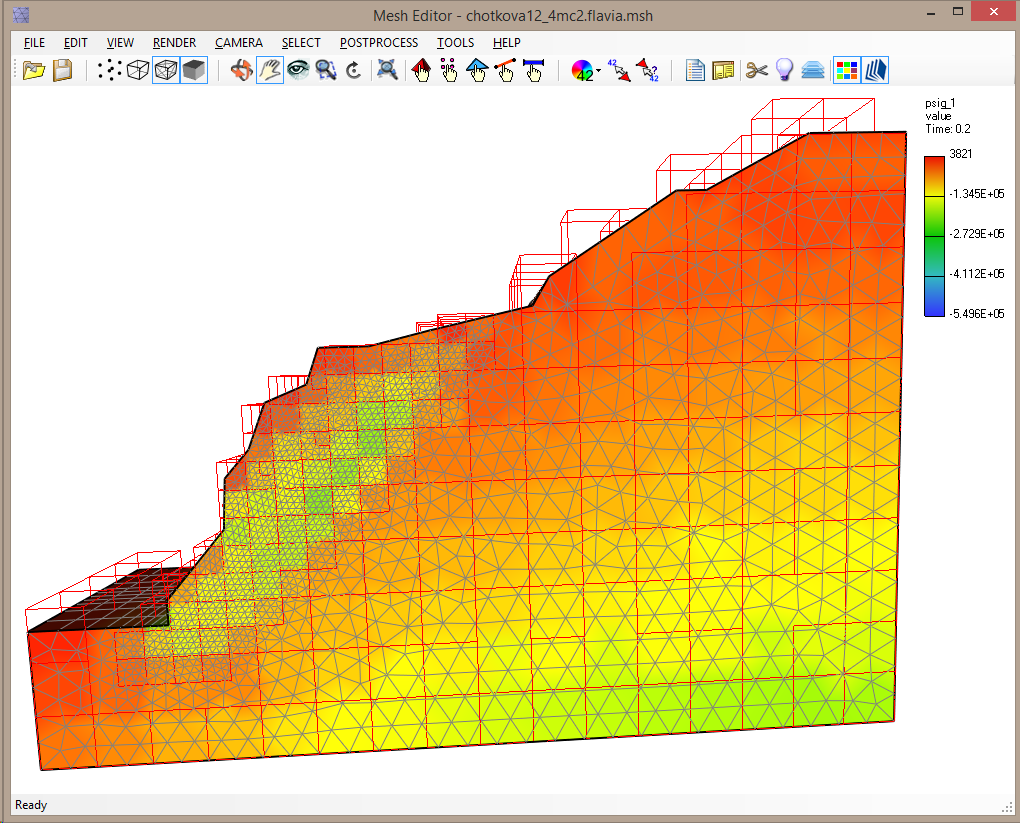
\includegraphics[width=\textwidth]{figures/chapter-approximation/figure10}
\decoRule
\caption[Mean value approximation of geological layers simulation results]{Geological layers simulation results. Mean value approximation of data values. Nodes in each cell have constant approximated value. High average error of an approximation. High memory consumption due to high average depth of the octree. Non-smooth transition between cells.}
\label{fig:geological-layers-mean}
\end{figure}

\begin{figure}[H]
\centering
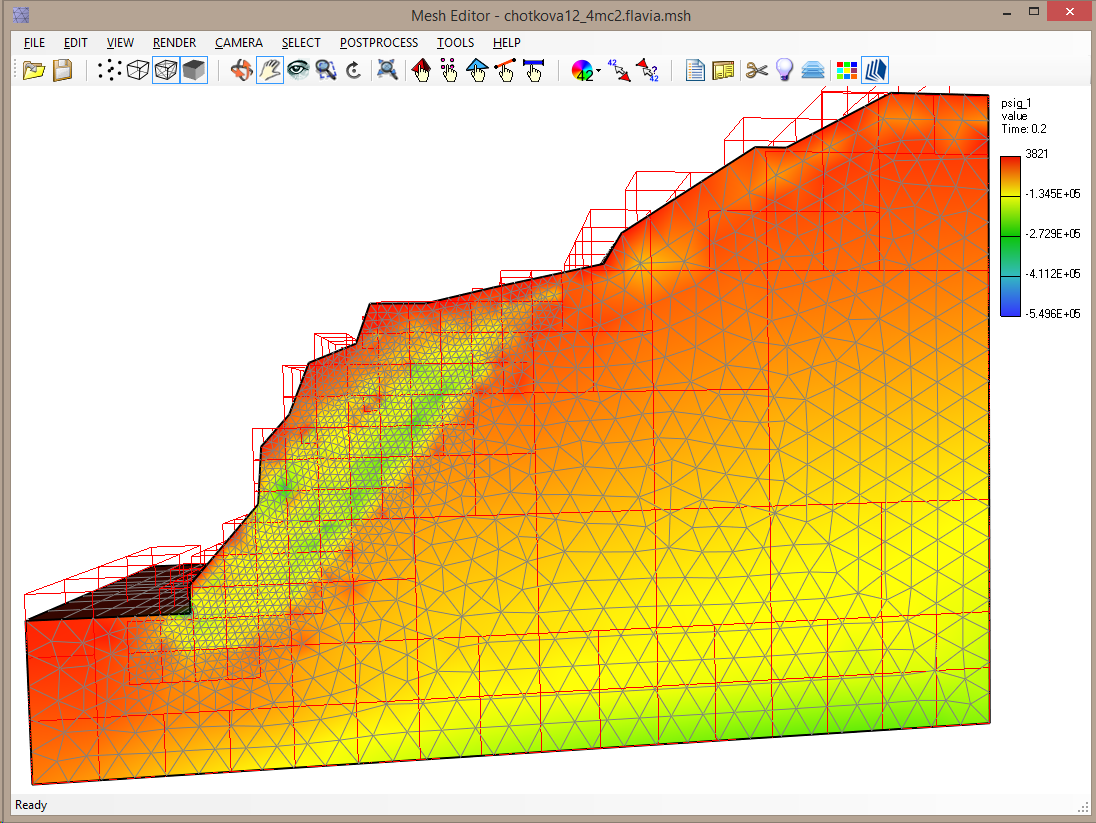
\includegraphics[width=\textwidth]{figures/chapter-approximation/figure11}
\decoRule
\caption[Trilinear approximation of geological layers simulation results]{Geological layers simulation results. Trilinear approximation of data values. Seamless transition between cells. Low depth of the octree in smooth areas. Can't capture high frequent changes in data which is common disadvantage of all lossy compressions.}
\label{fig:geological-layers-trilinear}
\end{figure}

Figure \ref{fig:geological-layers-exact} contains visualization of the exact data values whereas Figure \ref{fig:geological-layers-mean} and Figure \ref{fig:geological-layers-trilinear} contains visualization of approximation of the same data series but for different types of approximation functions to highlight the imperfections of the approximation algorithm. The red lines represent the octree cells.


%----------------------------------------------------------------------------------------
%	SUB-SECTION Approximation in time
%----------------------------------------------------------------------------------------

\subsection{Approximation in time}

Additional data compression can be gained by focusing on temporal dimension of function values. Memory allocation can be lowered by eliminating unimportant time steps. To achieve that, it is necessary to find those time steps, in which function values are steady or are changing linearly and can be therefore interpolated from other time steps.

Figure \ref{fig:interpolation-in-time} illustrates the idea of interpolation in time. Intermediate time steps can be interpolated from the key time steps if they have similar shape -- they are \textit{nearly} linear combinations of each other and therefore data in redundant time steps can be disposed. The decision whether to dispose time step or not is based on difference of two functions compared to experimentally designated threshold value. Mathematical background of this procedure is described later in this section.

\begin{figure}[H]
\centering
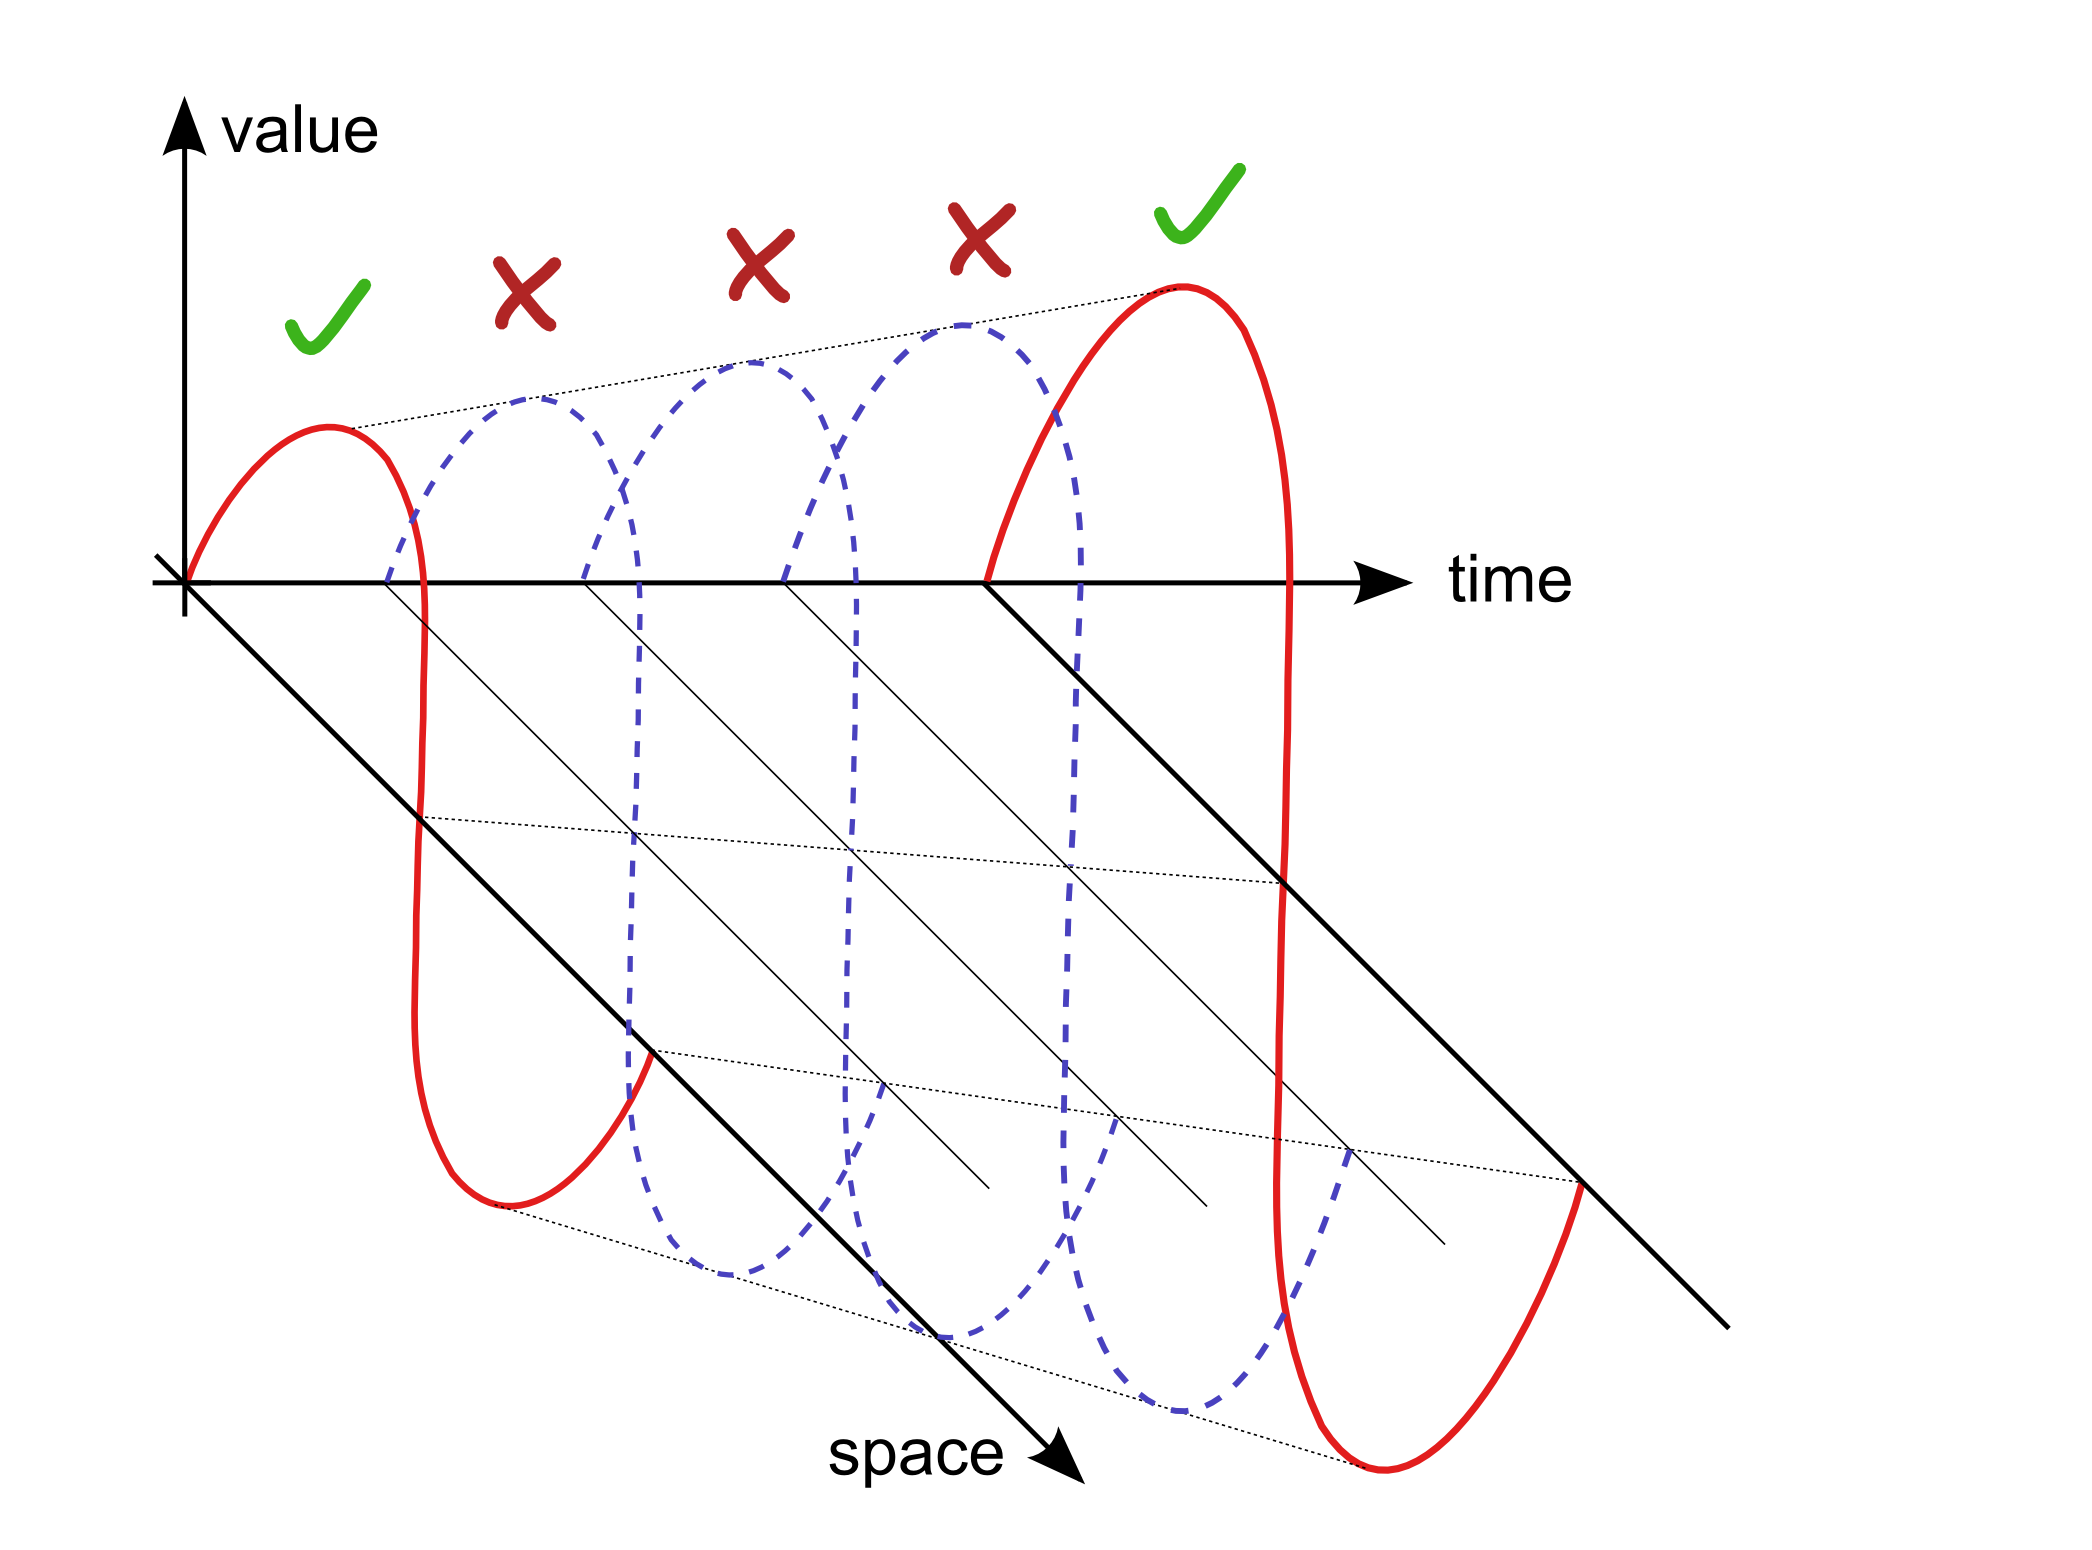
\includegraphics[width=\textwidth]{figures/chapter-approximation/figure12}
\decoRule
\caption[Interpolation in time diagram]{Interpolation in time. Intermediate time steps (blue) can be interpolated from the key time steps (red) if they have similar shape.}
\label{fig:interpolation-in-time}
\end{figure}

Several options to store temporal data were considered.

\begin{itemize}
  \item Sequence of octrees. Each one for single time step.
  \item 4D tree. Extension of octal tree on temporal dimension. Each internal node has 16 children.
  \item Single ordinary octree containing data approximations with time component. Extending the approximation functions by temporal dimension, e.g. quadrilinear form instead of trilinear form.
  \item Combination of octree for spatial decomposition and binary tree for temporal dimension division.
\end{itemize}

Octree for each time frame of an animation is memory inefficient as well as 4D tree \cite{Reilly2011}. 4D approximation functions have many parameters and also can’t capture intricate evolution of function in time. Therefore, different solution was suggested -- single octree representing spatial decomposition that is formed by merging sequence of octrees from all time steps. However, the sequence of octrees is just a virtual term. Algorithm 1 treats all data component from all time steps the same and when it finishes its job, only single octree is left with data approximation object for various data component and time steps stored in data catalog in each octree node independent to each other. By merging it is meant the unifying all time steps of a single data component in each octree node into single data sequence object that can be then a subject of the time compression algorithm. This process of merging virtual octrees for each time step into single ``time-tree'' is illustrated in Figure \ref{fig:unifying-time-steps}. Notice that the octree for each time step can have different structure and depth, because in each time step the original function can have different frequency spectrum for which the different sampling rate is needed.

\begin{figure}[H]
\centering
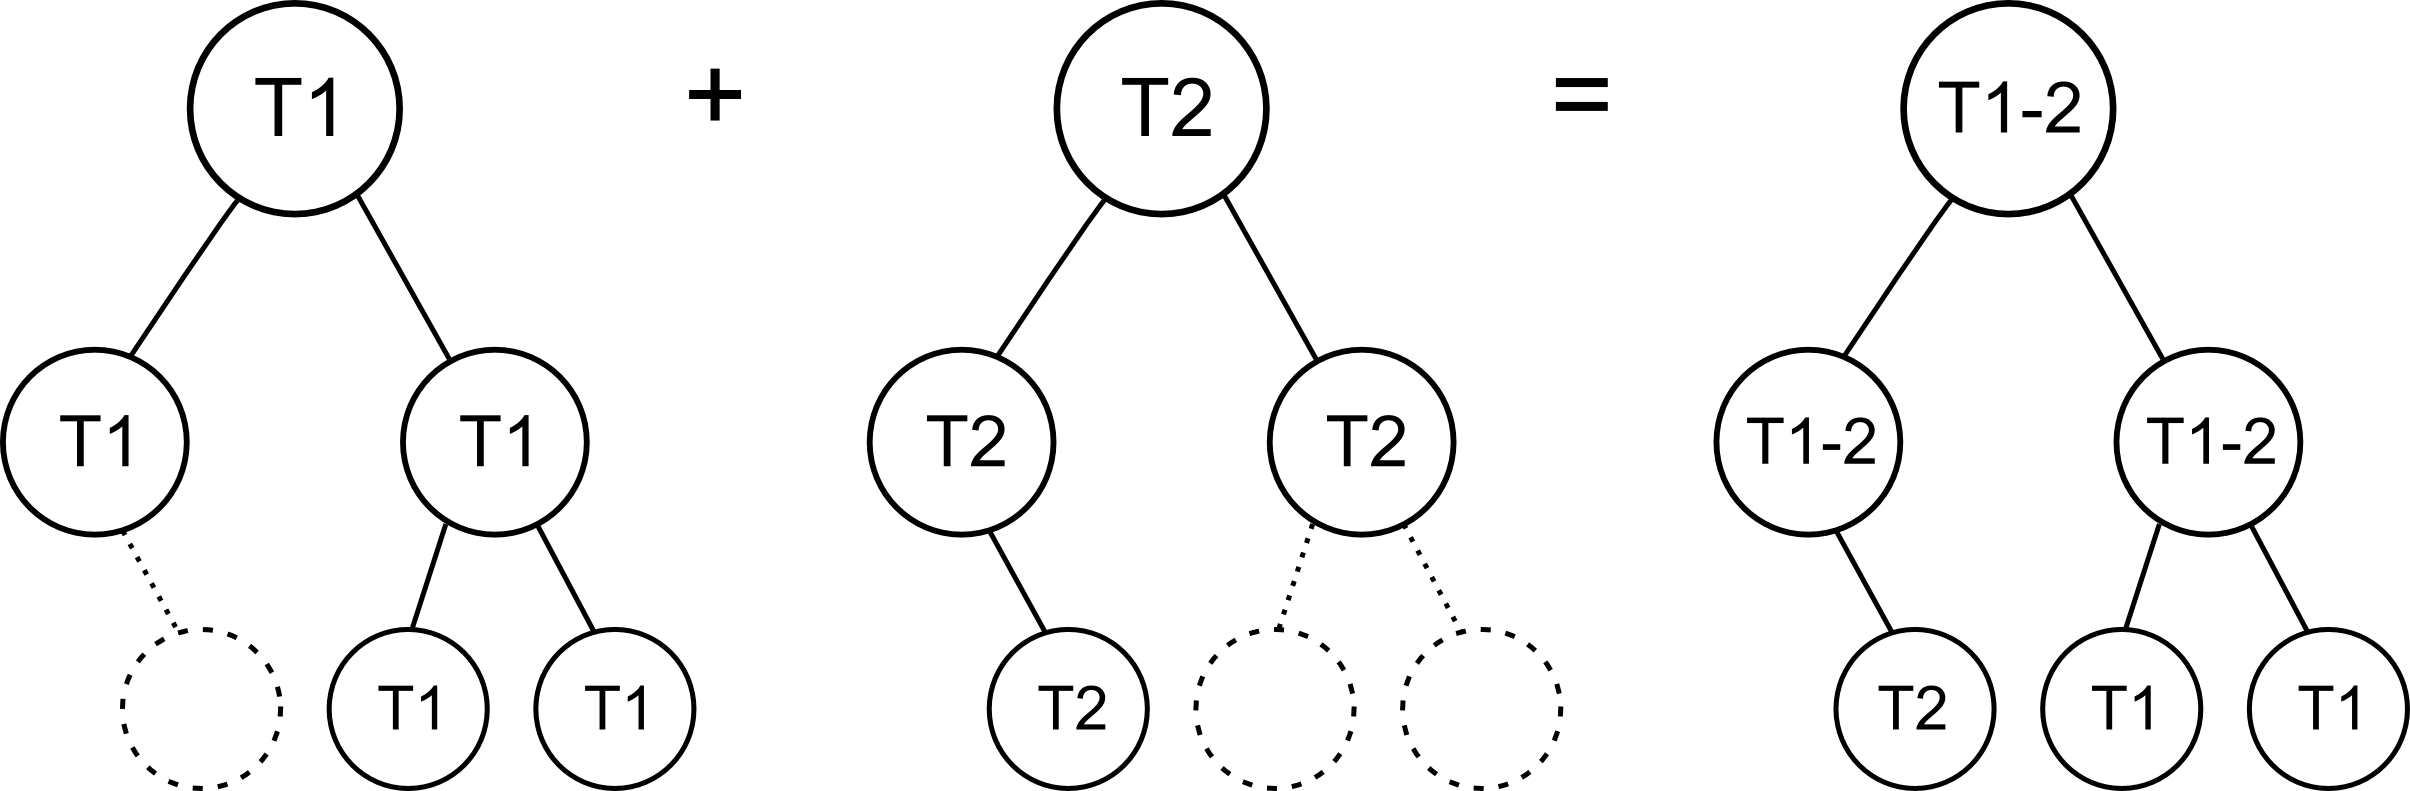
\includegraphics[width=\textwidth]{figures/chapter-approximation/figure13}
\decoRule
\caption[Illustration of unifying time steps in octree nodes]{Illustration of unifying time steps in octree nodes. For the sake of simplicity the binary tree is shown instead of octree. T1 and T2 represent approximation functions of the same data component in different time steps. Result of the union is single octree that contains sequences of corresponding time steps in its nodes.}
\label{fig:unifying-time-steps}
\end{figure}

However, not all approximation functions are preserved during merging. Each octree cell contains list of approximation functions only for key time steps, that are necessary to cover time development of discrete function in area represented by the octree cell. These key (or fixed) time steps are either specified by the user or identified automatically by the algorithm presented in Listing \ref{alg:approximation-in-time}.

Original nodal value retrieving is the same octree traversal as was depicted in Figure \ref{fig:nodal-value-computation} except for the final phase -- calculating value from approximation function in leaf octree nodes. If desired time instant is not present, then it must be interpolated from the key time steps. To find concrete time instant in the list of approximation functions the fast binary search algorithm is used.

Temporal-data-containing-octree is created by algorithm that works with already created octree having approximation functions for all time steps. At first it finds time steps that must be preserved. Those can be explicitly picked by the user or the algorithm itself determines automatically the first and the last time step as key times. Then the program traverses steps between key events of time interval. In each time step the algorithm iterates over space approximations for each loaded quantities and computes difference between each function and function created by interpolation of functions in key intervals. If this difference is lower than some preset fixed value, approximation function in current time step can be disposed because it can be created on demand in the future. Otherwise time interval is divided in current step and algorithm is recursively called on each of both intervals. It is therefore similar algorithm to approximation in space, but instead of octree a binary tree is used because there is only one temporal dimension instead of three spatial dimensions. Pseudo-code of approximation in time is shown in Listing \ref{alg:approximation-in-time}.

\begin{lstlisting}[caption=Approximation in time procedure,label=alg:approximation-in-time]
function compressTimeSteps(fromIndex, toIndex)
{
  // recursion stopping criterion
  if (toIndex - 1 <= fromIndex)
    return

  fromApproximation = timeSteps[fromIndex].Approximation
  toApproximation = timeSteps[toIndex].Approximation
  
  for (index = fromIndex + 1; index < toIndex; index++)
  {
    currentTime = timeSteps[index]
    timeFactor = (currentTime - timeSteps[fromIndex]) / (timeSteps[toIndex] - timeSteps[fromIndex])
    
    testFunction = timeSteps.Values[index].Approximation
    interpolatedFunction = InterpolatePolynomial(fromApproximation, toApproximation, timeFactor)

    sumDiffSqr = 0.0, sumFuncSqr = 0.0

    // compute difference of testFunction and interpolatedFunction
    foreach (testPoint in domainPoints)
    {
      testValue = testFunction.ComputeValue(testPoint)
      interpolatedValue = interpolatedFunction.ComputeValue(testPoint)
      diff = testValue - interpolatedValue
      
      sumDiffSqr += diff * diff
      sumFuncSqr += testValue * testValue
    }

    absoluteError = sqrt(sumDiffSqr)
    absoluteValue = sqrt(sumFuncSqr)
    relativeError = absoluteError / absoluteValue

    // if functions are not similar
    if (relativeError <= MAX_RELATIVE_ERROR)
    {
      // discard current time step
      removeTimeStep(currentTime)
    }
    else
    {
      half = (toIndex + fromIndex) / 2
      // recursive call on first half
      compressTimeSteps(fromIndex, half)
      // recursive call on second half
      compressTimeSteps(half, toIndex)
      return
    }
  }
}

// Approximation in time is called upon holes between fixed (key) time steps
// Fixed time steps are at least first and last time step and any interleaved time step specified by user
for (i = 1; i < fixedTimesIndexes.Count; i++)
{
  compressTimeSteps(fixedTimesIndexes[i - 1], fixedTimesIndexes[i])
}
\end{lstlisting}

In the case of approximation in time, we have two continuous functions that we want to compare to each other. First function is approximation function for the time step that can be potentially removed. This function is already created by spatial approximation algorithm described above. Second function is computed ad-hoc from key time steps to test if it can potentially replace the first function later. If the test succeeds (functions are similar enough) the first function can be removed entirely from octree data structure, because it can be computed from the functions in neighboring time steps.

The process of computing intermediate function from the key time steps is quite straightforward. With regard to the fact that all approximation functions have to be of the same polynomial type, each parameter of the interpolated function can be then computed as interpolation of the related parameters in two boundary functions in key time steps.

Approximation in time is made for each spatial octree node separately instead of globally for the whole mesh, because the quantity can change in time only in some parts of the mesh and in others can be constant.

%----------------------------------------------------------------------------------------
%	SUB-SUB-SECTION Difference between two functions
%----------------------------------------------------------------------------------------

\subsubsection{Difference between two functions}

The algorithm for approximation in time has to compare two continuous approximation functions to determine their similarity.

The difference $d$ of two continuous square-integrable functions $u$ and $v$ is considered as scalar value computed as

\begin{equation}
  d = \sqrt{\int_{\Omega}(u-v)^2 \diff\Omega}.
\end{equation}

If $u \neq 0$ relative difference $\hat{d}$ is then

\begin{equation}
  \hat{d} = \frac{\sqrt{\int_{\Omega}(u-v)^2\diff\Omega}}{\sqrt{\int_{\Omega}u^2\diff\Omega}}.
\end{equation}

To move from continuous to discrete world the integrals can be replaced by sums

\begin{equation}
  \int_{\Omega}f(x)\diff x = \sum_{i=1}^{m}f(x_i) w_i,
\end{equation}

where $w_i$ is the weight of the $i$-th test point with the meaning of volume surrounding the point, $x_i$ is the location of the test point and $m$ is the number of integration points. The test points in the formula are the data points situated in the area represented by approximation function $f$ in the presented algorithm.

Relative error $\tilde{d}$ is then

\begin{equation}
  \tilde{d} = \sqrt{\frac{\sum_{i=1}^{m}(u(x_i)-v(x_i))^2 w_i}{\sum_{i=1}^{m}u(x_i)^2 w_i}}.
\end{equation}

The value of $\tilde{d}$ is then compared to $\epsilon$ value. The value $\epsilon=0.001$ came from the experiments as the best-fitting value. If condition $\tilde{d} \leq \epsilon$ holds, functions $u$ and $v$ are considered equal in terms of approximation in time. The value $\epsilon$ matches \code{MAX\_RELATIVE\_ERROR} parameter in Listing \ref{alg:approximation-in-time}.

%----------------------------------------------------------------------------------------
%	SUB-SUB-SECTION Results
%----------------------------------------------------------------------------------------

\subsubsection{Results}

Results of the approximation in time are summarized in Table \ref{tab:reactor-vessel-spacetime}. For spatial approximation the trilinear regression was chosen as the method with the best results in the previous benchmark. The reactor vessel simulation results were used in the test (see Figure \ref{fig:reactor-vessel-displacements}).

\begin{table}[H]
\caption[Approximated results of reactor vessel 2D simulation (space and time)]{Reactor vessel 2D. Spatial and temporal octree approximation results.}
\label{tab:reactor-vessel-spacetime}
\centering
\begin{tabular}{| l | r | r | r |}
\hline
\tabhead{ } & \tabhead{Max error [\%]} & \tabhead{Average error [\%]} & \tabhead{Compression ratio [\%]} \\
\hline
Mean value & 100.7 \textcolor{negativeColor}{(+25.42)} & 0.7835 \textcolor{negativeColor}{(+0.16)} & 7.53 \textcolor{positiveColor}{(-47.77)}\\
Linear regression & 44.23 \textcolor{neutralColor}{(+0.0)} & 0.2262 \textcolor{negativeColor}{(+0.042)} & 2.57 \textcolor{positiveColor}{(-15.13)}\\
Trilinear regression & 81.41 \textcolor{negativeColor}{(+0.14)} & 0.2158 \textcolor{negativeColor}{(+0.041)} & 2.54 \textcolor{positiveColor}{(-14.34)}\\
\hline
\end{tabular}
\end{table}

Time compression procedure presented in Listing \ref{alg:approximation-in-time} was applied to already created octree-based structure containing approximations of original data values. Generation of this octree is described in section \ref{sec:approximation-in-space}.

\todo{TODO: add results evaluation from papers \cite{Benes2016} and \cite{Benes2016Pollack}}